% Options for packages loaded elsewhere
\PassOptionsToPackage{unicode}{hyperref}
\PassOptionsToPackage{hyphens}{url}
\PassOptionsToPackage{dvipsnames,svgnames,x11names}{xcolor}
%
\documentclass[
]{article}
\usepackage{amsmath,amssymb}
\usepackage{iftex}
\ifPDFTeX
  \usepackage[T1]{fontenc}
  \usepackage[utf8]{inputenc}
  \usepackage{textcomp} % provide euro and other symbols
\else % if luatex or xetex
  \usepackage{unicode-math} % this also loads fontspec
  \defaultfontfeatures{Scale=MatchLowercase}
  \defaultfontfeatures[\rmfamily]{Ligatures=TeX,Scale=1}
\fi
\usepackage{lmodern}
\ifPDFTeX\else
  % xetex/luatex font selection
\fi
% Use upquote if available, for straight quotes in verbatim environments
\IfFileExists{upquote.sty}{\usepackage{upquote}}{}
\IfFileExists{microtype.sty}{% use microtype if available
  \usepackage[]{microtype}
  \UseMicrotypeSet[protrusion]{basicmath} % disable protrusion for tt fonts
}{}
\makeatletter
\@ifundefined{KOMAClassName}{% if non-KOMA class
  \IfFileExists{parskip.sty}{%
    \usepackage{parskip}
  }{% else
    \setlength{\parindent}{0pt}
    \setlength{\parskip}{6pt plus 2pt minus 1pt}}
}{% if KOMA class
  \KOMAoptions{parskip=half}}
\makeatother
\usepackage{xcolor}
\usepackage[left=2cm,right=2cm,top=2cm,bottom=2cm]{geometry}
\usepackage{longtable,booktabs,array}
\usepackage{calc} % for calculating minipage widths
% Correct order of tables after \paragraph or \subparagraph
\usepackage{etoolbox}
\makeatletter
\patchcmd\longtable{\par}{\if@noskipsec\mbox{}\fi\par}{}{}
\makeatother
% Allow footnotes in longtable head/foot
\IfFileExists{footnotehyper.sty}{\usepackage{footnotehyper}}{\usepackage{footnote}}
\makesavenoteenv{longtable}
\usepackage{graphicx}
\makeatletter
\def\maxwidth{\ifdim\Gin@nat@width>\linewidth\linewidth\else\Gin@nat@width\fi}
\def\maxheight{\ifdim\Gin@nat@height>\textheight\textheight\else\Gin@nat@height\fi}
\makeatother
% Scale images if necessary, so that they will not overflow the page
% margins by default, and it is still possible to overwrite the defaults
% using explicit options in \includegraphics[width, height, ...]{}
\setkeys{Gin}{width=\maxwidth,height=\maxheight,keepaspectratio}
% Set default figure placement to htbp
\makeatletter
\def\fps@figure{htbp}
\makeatother
\setlength{\emergencystretch}{3em} % prevent overfull lines
\providecommand{\tightlist}{%
  \setlength{\itemsep}{0pt}\setlength{\parskip}{0pt}}
\setcounter{secnumdepth}{-\maxdimen} % remove section numbering
\usepackage{wrapfig}
\usepackage{graphicx}
\usepackage{titlesec}
\titlespacing*{\section}{0pt}{\baselineskip}{0\baselineskip}
\titlespacing*{\subsection}{0pt}{\baselineskip}{0\baselineskip}
\titlespacing*{\subsubsection}{0pt}{\baselineskip}{0\baselineskip}
\usepackage{fancyhdr}
\pagestyle{fancy}
\fancyhf{}
\fancyfoot[R]{}
\renewcommand{\headrulewidth}{0pt}
\usepackage{etoolbox}
\usepackage{array}
\AtBeginEnvironment{table}{\vspace{-0.3\baselineskip}}
\ifLuaTeX
  \usepackage{selnolig}  % disable illegal ligatures
\fi
\usepackage{bookmark}
\IfFileExists{xurl.sty}{\usepackage{xurl}}{} % add URL line breaks if available
\urlstyle{same}
\hypersetup{
  colorlinks=true,
  linkcolor={Maroon},
  filecolor={Maroon},
  citecolor={Blue},
  urlcolor={blue},
  pdfcreator={LaTeX via pandoc}}

\author{}
\date{\vspace{-2.5em}}

\begin{document}

\pagenumbering{gobble}

To,

Professor Jeffrey W. Doser

Statistical Ecology and Forest Science Lab

North Carolina State University

\href{mailto:doserjef@msu.edu}{\nolinkurl{doserjef@msu.edu}}

\begin{centering}

\vspace{0.5cm}

\bf{Ref: Cover Letter for PhD position in Statistical Ecology or Quantitative Forest Science}

\end{centering}

I am writing to express my interest in the PhD position in Statistical
Ecology or Quantitative Forest Science lab in the Department of Forestry
and Environmental Resources at North Carolina State University. I hold a
Master's degree in Landscape Ecology and Nature Conservation from the
University of Greifswald, Germany, and a Bachelor's degree in Forestry
from Tribhuvan University, Nepal. My academic journey has equipped me
with a foundation in ecological principles, statistical computing and
research methodologies. Additionally, I have enhanced my capacity with
key skills in data science and programming knowledge particularly using
R and Python.

I have an experience of working at Forest Research and Training Center
for more than eight years where, major responsibilities included
national forest inventory and data analysis, tree biometrics and some
application of remote sensing and GIS. Recently, I am working as a
Research Officer at the Ministry of Forests and Environment, Nepal. In
this role, I have been actively involved in preparing national GHG
inventory reports My professional experience further motivated me to
understand problems ranging from simple tree level computing to
understanding spatial and temporal ecological processes over larger
territories.

In past couple of years, I am keen on learning statistical ecology and
its practical application in forestry sector. While conducting national
level inventory and data collection, many stakeholders seek method to
interpolate those estimation to regional and local scale which has been
a challenge for me. Since 2021, I am learning data science, statistical
computing, machine learning algorithms and its application in
environmental sector. I have been instructing non graduate and graduate
students on R programming, data manipulation, data visualization and
statistical analysis which significantly boosted my programming skills
and gave me confidence on solving computational problems. I have been
following the Inferential Statistics, Bayesian Statistics and its
application but due to lack of sufficient experience I have not yet been
able to apply these concepts to solve the research problems. Recently,
while seeking an opportunity to work on an academic environment to focus
on learning and applying quantitative / statistical ecology, I came
across this announcement for graduate position.

I am eager to pursue a PhD in Statistical Ecology or Quantitative Forest
Science because it perfectly aligns with my professional aspirations and
research interests. My extensive experience in forest inventory, data
analysis, has exposed me to the pressing challenges in forestry and
environmental management, particularly the need for robust statistical
models to inform decision-making at various spatial scales. This has
driven me to deepen my expertise in statistical ecology and its
application in forestry. Broadly, research areas offered by your lab
aligns with my research interest, but I am particularly interested in
the development of statistical models to understand ecological processes
across macroscales and small area estimation of forest parameters. I am
particularly drawn to your lab's focus on deepening understanding of
statistical methods, including Bayesian approaches, as they provide a
powerful foundation to complement frequentist explanations with prior
knowledge, ultimately improving model accuracy.

Enclosed is my CV, which provides further details about my
qualifications and achievements. I look forward to the opportunity to
discuss how my skills and experiences align with the goals of the
project.

Thank you for considering my application.

\vspace{1cm}

\begin{figure}[h]
    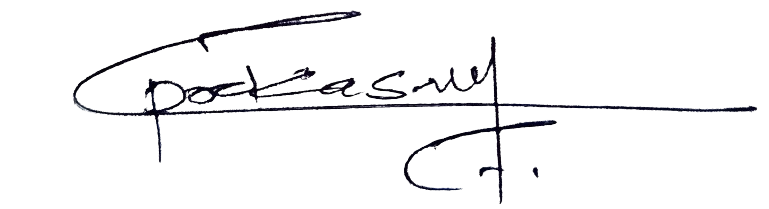
\includegraphics[width=1in, height=2in]{sign.png}
\end{figure}

\textbf{Prakash Lamichhane}

\textbf{\emph{18 September 2024}}

\newpage 
\Huge

\bf{PRAKASH LAMICHHANE}

\par

\normalsize
\mdseries

\bf{Research Officer/Data Ananlyst/Ecologist}

\par

\normalsize
\mdseries

Email:
\href{mailto:forester.prakash@gmail.com}{\nolinkurl{forester.prakash@gmail.com}}
\textbar{} Phone: +977-9845228896 \textbar{} GitHub:
\href{https://github.com/foresterprakash}{foresterprakash} \textbar{}
LinkedIn:
\href{https://www.linkedin.com/in/PrakashLamichhane}{PrakashLamichhane}
\textbar{} ORCID:
\href{https://orcid.org/0000-0002-0355-0222}{0000-0002-0355-0222}
\textbar{}

\section{\texorpdfstring{\underline{Education and Awards}}{}}\label{section}

\begin{longtable}[]{@{}
  >{\raggedright\arraybackslash}p{(\columnwidth - 6\tabcolsep) * \real{0.1375}}
  >{\raggedright\arraybackslash}p{(\columnwidth - 6\tabcolsep) * \real{0.4875}}
  >{\raggedright\arraybackslash}p{(\columnwidth - 6\tabcolsep) * \real{0.2750}}
  >{\raggedright\arraybackslash}p{(\columnwidth - 6\tabcolsep) * \real{0.1000}}@{}}
\toprule\noalign{}
\endhead
\bottomrule\noalign{}
\endlastfoot
Sept.~2024 & Distinguished Speaker Award &
\href{https://igckorea.kr/theme/grape/mobile/sub01_05.php}{GIR} &
Korea \\
2017 & DAAD ScholarShip Award & For Masters Study & Germany \\
2017 - 2019 & M.Sc. Landscape Ecology and Nature Conservation &
University of Greifswald & Germany \\
2010 - 2013 & B.Sc. Forestry & Tribhuvan University & Nepal \\
2007 - 2009 & Technical Level in Forestry (I.Sc.) & Tribhuvan University
& Nepal \\
\end{longtable}

\section{\texorpdfstring{\underline{Work Experiences}}{}}\label{section-1}

\begin{longtable}[]{@{}
  >{\raggedright\arraybackslash}p{(\columnwidth - 2\tabcolsep) * \real{0.1867}}
  >{\raggedright\arraybackslash}p{(\columnwidth - 2\tabcolsep) * \real{0.8133}}@{}}
\toprule\noalign{}
\endhead
\bottomrule\noalign{}
\endlastfoot
2017 - 2019 & M.Sc. Landscape Ecology and Nature Conservation,
Greifswald University \\
2019 - 2023 & Assistant Research Officer, Forest Survey and Carbon
Monitoring Section under FRTC \\
2023 - Present & Research Officer, Climate Change Management Division,
MOFE \\
Part-time & Lecturer, Natural Resource Economics, Kathmandu Forestry
College \\
\end{longtable}

\section{\texorpdfstring{\underline{Research Experience}}{}}\label{section-2}

\begin{itemize}
\item
  Preparation of National Landcover monitoring System (NLCMS) using
  RandomForestClassifier.
\item
  FRTC, 2020, A study of Opportunities and Constraints for Development
  of Private forestry Model in Mid-Hill Region of Nepal (A case study
  from Kavre and Kaski district of Nepal), Forest Research and Training
  Centre (FRTC), Babarmahal, Kathmandu, Nepal.
  \href{https://frtc.gov.np/uploads/files/Private\%20forest\%20Model(1).pdf}{Unpublished}
\item
  Preparation of Regional and National Forest Resource assessment
  (Involvement in field data collection, data analysis and report
  writing).
\item
  Involvement in generating activity data and emission factors for
  national emission reduction report for MRV purpose in coordination
  with FCPF and World Bank.
\end{itemize}

\section{\texorpdfstring{\underline{Publications}}{}}\label{section-3}

\begin{itemize}
\item
  Aryal, S., Paudel, P., Bolakhe, S., Mahatara, D., \&
  \textbf{Lamichhane, P}. (2022). Evaluation of error and efficiency on
  tree height measurement using Abney's level, Rangefinder and Vertex
  IV. \emph{Indian Journal of Forestry}, 45(1), 1--8.
  \href{https://doi.org/10.54207/bsmps1000-2022-49P4F8}{DOI}
\item
  Parajuli, A., Gautam, A. P., Sharma, S., \textbf{Lamichhane, P}.,
  Sharma, G., Bist, B. S., Aryal, U., \& Basnet, R. (2022). A Strategy
  for involving community forest managers in effective forest fire
  management in Nepal. \emph{Banko Janakari}, 32(1), 41--51.
  \href{https://doi.org/10.3126/banko.v32i1.45476}{DOI}
\item
  Subedi, B., \textbf{Lamichhane, P}., Magar, L. K., \& Subedi, T.
  (2022). Aboveground carbon stocks and sequestration rates of forests
  under different management regimes in Churia region of Nepal.
  \emph{Banko Janakari}, 32(1), 15--24.
  \href{https://doi.org/10.3126/banko.v32i1.45442}{DOI}
\item
  Gautam, G. P., Aryal, R. R., \& \textbf{Lamichhane, P}. (2018).
  Restoration of degraded land through Moso bamboo (Phyllostachys
  pubescens) plantation in the Mid-hills of Nepal. \emph{Banko
  Janakari}, 150--153.
  \href{https://doi.org/10.3126/banko.v27i3.20560}{DOI}
\item
  Dhakal, R., et al.~(2023). Developing Stem Taper of Shorea Robusta in
  the Far-Western Terai of Nepal. \emph{Banko Janakari}, 33(2), 3--10.
  \href{https://doi.org/10.3126/banko.v33i2.58809}{DOI}
\end{itemize}

\section{\texorpdfstring{\underline{Workshop and Seminar}}{}}\label{section-4}

\begin{itemize}
\tightlist
\item
  \textbf{July 2022}

  \begin{itemize}
  \tightlist
  \item
    Cross Country knowledge Exchange on REDD plus program in Cambodia
    dated from 12/06/2022 to 19/06/2022 Phnom Penn, Siem Reip and Koh
    Kong province of Cambodia (ORAL PRESENTATION)
  \end{itemize}
\item
  \textbf{December 2022}

  \begin{itemize}
  \tightlist
  \item
    South-South Knowledge Exchange on Measurement, Monitoring, Reporting
    and Verification systems, FCPF CF ERPA Implementation dated from
    12/12/2022 -- 18/12/2022 -- Maputo, Mozambique.
  \end{itemize}
\item
  \textbf{March 2024}

  \begin{itemize}
  \tightlist
  \item
    Hands-on training workshop on transitioning to the ETF, including
    the preparation of the Biennial Transparency Report for Asia Region
    dated from 12/03/2024 to 15/03/2024 Singapore.
  \end{itemize}
\item
  \textbf{June 2024}

  \begin{itemize}
  \tightlist
  \item
    UN Climate Conference Bonn, Germany dated from 03/06/2024 to
    09/06/2024
  \end{itemize}
\item
  \textbf{September 2024}

  \begin{itemize}
  \tightlist
  \item
    International Greenhouse Gas Inventory (IGC), 4 september 2024,
    Seoul organized by Greenhouse Gas Inventory and Research Center,
    Korea \textbf{(Distinguished Speaker Aaward)}
  \end{itemize}
\end{itemize}

\section{\texorpdfstring{\underline{Major Skills}}{}}\label{section-5}

\begin{itemize}
\tightlist
\item
  National Forest data analysis and Reporting
\item
  Mastering MS. Excel and R programming
\item
  Carbon accounting and MRV process
\item
  Uncertainty Estimation and Sensitivity Analysis
\item
  Data Science with Python
\item
  GIS Tools (QGIS, ARCGIS, Google Earth Engine etc.)
\item
  Integrated Development Environments (IDEs)(i.e., R Studio, VS code,
  Pycharm, Jupyter Notebook, Collect Earth Online etc.).
\end{itemize}

\section{\texorpdfstring{\underline{References}}{}}\label{section-6}

\begin{itemize}
\item
  \textbf{Shiva Khanal PhD,Western Sydney University,Australia} Ministry
  of Forests and Environment, Kathmandu, Nepal,\textbf{Email:}
  \href{mailto:khanalshiva1@gmail.com}{\nolinkurl{khanalshiva1@gmail.com}},\textbf{Phone:}
  (+977) 9841492155
\item
  \textbf{Shes Kanta Bhandari PhD, University of Western Australia}
  Assistant Professor, Institute of Forestry, Tribhuvan University,
  \textbf{Email:}
  \href{mailto:shes.bhandari@pc.tu.edu.np}{\nolinkurl{shes.bhandari@pc.tu.edu.np}},
  \textbf{Phone:} (+977) 9765631067
\item
  \textbf{Prof.~Martin Wilmking, Ph.D.~Professorship Landscape Ecology}
  Soldmannstr. 15, Room 1.37, University of Greifswald,\textbf{Email:}
  \href{mailto:wilmking@uni-greifswald.de}{\nolinkurl{wilmking@uni-greifswald.de}},
  \textbf{Phone:} +49 (0) 3834-4204095
\end{itemize}

\newpage

\section{\texorpdfstring{\underline{Trainings as Trainee}}{}}\label{section-7}

\begin{itemize}
\tightlist
\item
  \textbf{23-27 May, 2022}

  \begin{itemize}
  \tightlist
  \item
    Training on Unbiased Area Estimation and Uncertainty Estimation for
    Forest Activity Data, USAID, USFS, SilvaCarbon
    \href{https://crystal-wespestad.com/}{Crystal Westespad}
  \end{itemize}
\item
  \textbf{22- 26 August, 2022}

  \begin{itemize}
  \tightlist
  \item
    Development of National Landcover Monitoring System for Nepal,
    International Center for Integrated Mountain Development (ICIMOD)
    SERVIR-HKH initiative,
    \href{https://www.icimod.org/team/kabir-uddin}{kabir Uddin}
  \end{itemize}
\item
  \textbf{10 October - 11 November, 2022}

  \begin{itemize}
  \tightlist
  \item
    On the Job training on Forest Carbon Stock Measurement using Earth
    Observation Data, International Center for Integrated Mountain
    Development (ICIMOD) SERVIR-HKH initiative,
    \href{https://www.icimod.org/team/rajesh-bahadur-thapa/}{Rajesh
    Bahadur Thapa}
  \end{itemize}
\item
  \textbf{12 May - 13 August 2023}

  \begin{itemize}
  \tightlist
  \item
    Data Science with
    Python,\href{https://broadwayinfosys.com/}{Broadways Infosys
    Pvt.Ltd.},\href{https://www.linkedin.com/in/uttam-adhikari-30a53660/?originalSubdomain=np}{Uttam
    Adhikari}
  \end{itemize}
\item
  \textbf{21- 25 January 2024}

  \begin{itemize}
  \tightlist
  \item
    FCPF and ART TREES: Technical Training Workshop on REDD+ Emission
    Reduction Measurement, Reporting and Verification
    (30hours),\href{https://redd.gov.np/}{REDD + Implemmentation
    center},\href{https://www.silvacarbon.org/}{SilvaCarbon},
    \href{https://www.forestcarbonpartnership.org/sites/default/files/documents/nepal_ermr_ghg_accounting_nov_2023_final.pdf}{FCPF},
    \href{https://www.worldbank.org/en/home}{The WorldBank Group
    Nepal},\href{https://www.linkedin.com/in/german-obando-vargas-24b70319/?originalSubdomain=cr}{German
    Obando - Vargas}
  \end{itemize}
\item
  \textbf{22-26 July 2024}

  \begin{itemize}
  \tightlist
  \item
    Earth Observation (LiDAR and GEDI) for forest carbonstocks
    monitoring in Nepal, ICIMOD,
    FRTC,SilvaCarbon,\href{https://www.icimod.org/team/rajesh-bahadur-thapa/}{Rajesh
    Bahadur Thapa} and
    \href{https://www.linkedin.com/in/timothy-devereux/}{Tim Devereux}
  \end{itemize}
\item
  \textbf{19 Aug - 6 September 2024}

  \begin{itemize}
  \tightlist
  \item
    Climate Action and Support Transparency Training(CASTT) Programme on
    GHGs in Seoul,Republic of Korea,\textbf{UNFCCC}and Green House Gas
    Inventory and Research Center, South Korea,
    \href{https://www.linkedin.com/in/eunhae-jeong-248a40124/}{Jeong
    Eun-hae,President, GIR Korea}
  \end{itemize}
\end{itemize}

\section{\texorpdfstring{\underline{Trainings as Trainer}}{}}\label{section-8}

\begin{itemize}
\tightlist
\item
  \textbf{Regular From 2022}

  \begin{itemize}
  \tightlist
  \item
    MS Excel and R Programming Trainer in
    \href{https://broadwayinfosys.com/}{Broadways Infosys}
  \end{itemize}
\item
  \textbf{14 - 21 Aug, 2023}

  \begin{itemize}
  \tightlist
  \item
    Training on Python Programming, \href{https://frtc.gov.np/}{Forest
    Research and TRaining Center}
  \end{itemize}
\item
  \textbf{26 Sept - 5 Oct, 2023}

  \begin{itemize}
  \tightlist
  \item
    Statistical Data Analysis and Forest Mapping,
    \href{https://frtc.gov.np/}{Forest Research and Training Center}
  \end{itemize}
\item
  \textbf{4-13 Feb, 2024}

  \begin{itemize}
  \tightlist
  \item
    Enhancing Capacity on R Programming for Data Analysis and Carbon
    Accounting, \href{https://redd.gov.np/}{REDD+ Implementation center}
  \end{itemize}
\end{itemize}

\end{document}
